\documentclass[9pt]{beamer}

% Packages
\usepackage{amsmath, amssymb, amsthm}
\usepackage{graphicx}
\usepackage{booktabs}
\usepackage{listings}
\usepackage{xcolor}
\usepackage{hyperref}
\usepackage{tikz}
\usepackage{mathtools}
\usepackage{tcolorbox}
\usepackage{listingsutf8}
\usetikzlibrary{arrows,shapes,matrix,positioning}
% Theme setup
\usetheme{Madrid}
\usecolortheme{dolphin}
\setbeamertemplate{navigation symbols}{}
\setbeamertemplate{blocks}[rounded][shadow=true]

% Code listings setup
\lstset{
    basicstyle=\tiny\ttfamily\small,
    breaklines=true,
    commentstyle=\color{green!50!black},
    keywordstyle=\color{blue},
    stringstyle=\color{red},
    numberstyle=\tiny\color{gray},
    backgroundcolor=\color{gray!10},
    frame=single,
    rulecolor=\color{black!30},
    captionpos=b,
    escapeinside={(*@}{@*)},
    extendedchars=true,
}

% Define colors for tips and notes
\definecolor{tipcolor}{RGB}{0,128,0}
\definecolor{warningcolor}{RGB}{204,102,0}

% Custom environments
\newenvironment{tip}{\begin{tcolorbox}[colback=green!10,colframe=green!50!black,title=Tip]}{\end{tcolorbox}}
\newenvironment{practice}{\begin{tcolorbox}[colback=blue!10,colframe=blue!50!black,title=Hands-on Practice]}{\end{tcolorbox}}
\newenvironment{warning}{\begin{tcolorbox}[colback=orange!10,colframe=orange!50!black,title=Common Mistake]}{\end{tcolorbox}}

\title{\LaTeX: introduction}
\subtitle{Multi-session mini workshop}
\author{Morteza Maleki}
\institute{Tarbiat Modares University}
\date{\today}

\begin{document}
    
    %------------------------------------------------
    % Title slide
    %------------------------------------------------
    \begin{frame}
        \titlepage
    \end{frame}
    
    %------------------------------------------------
	% session 00: Overview
    %------------------------------------------------

    
%------------------------------------------------
% Workshop Overview
%------------------------------------------------
\begin{frame}{Workshop Overview}
	\begin{columns}
		\begin{column}{0.5\textwidth}
			\textbf{Hour 1:} Getting Started
			\begin{itemize}
				\item What is LaTeX?
				\item Basic document structure
				\item Text formatting
			\end{itemize}
			
			\textbf{Hour 2:} Mathematical Typesetting
			\begin{itemize}
				\item Inline \& display math
				\item Essential math commands
				\item Matrices and equation alignment
			\end{itemize}
		\end{column}
		
		\begin{column}{0.5\textwidth}
			\textbf{Hour 3:} Document Structure
			\begin{itemize}
				\item Theorems and proofs
				\item Figures and tables
				\item Cross-referencing
			\end{itemize}
			
			\textbf{Hour 4:} Advanced Topics
			\begin{itemize}
				\item Bibliography basics
				\item Useful packages
				\item Debugging and resources
			\end{itemize}
		\end{column}
	\end{columns}
\end{frame}

%------------------------------------------------
% Workshop Learning Goals
%------------------------------------------------
\begin{frame}{Learning Goals}
	By the end of this workshop, you will be able to:
	\begin{itemize}
		\item Write basic LaTeX documents from scratch
		\item Typeset complex mathematical expressions professionally
		\item Structure mathematical papers and notes with proper sections
		\item Include figures, tables, and bibliographic references
		\item Debug common LaTeX errors
		\item Know where to find further resources
	\end{itemize}
\end{frame}

%------------------------------------------------
% Preparation Requirements
%------------------------------------------------
\begin{frame}{Preparation \& Requirements}
	\begin{block}{Please install before we begin:}
		\begin{itemize}
			\item A TeX distribution:
			\begin{itemize}
				\item Windows: MiKTeX or TeX Live
				\item macOS: MacTeX
				\item Linux: TeX Live
			\end{itemize}
			\item A LaTeX editor:
			\begin{itemize}
				\item TeXworks (included with most distributions)
				\item TeXstudio (recommended for beginners)
				\item Or create an \textbf{Overleaf.com} account (web-based, preferred)
			\end{itemize}
		\end{itemize}
	\end{block}
	
	\begin{alertblock}{Workshop Materials}
		\begin{itemize}
			\item Example .tex files (download provided link)
			\item LaTeX math cheatsheet
			\item These slides (will be shared after the workshop)
			\item Problems (+ Solutions afterward)
		\end{itemize}
	\end{alertblock}
\end{frame}

    %------------------------------------------------
    % session 01: GETTING STARTED WITH LATEX
    %------------------------------------------------
    
\section{Getting Started with LaTeX}

\begin{frame}{What is LaTeX?}
    \begin{columns}
        \begin{column}{0.6\textwidth}
            \begin{itemize}
                \item A document preparation system using markup language
                \item Pronounced "Lay-tech" or "Lah-tech"
                \item Created by Leslie Lamport (based on TeX by Donald Knuth)
                \item Focuses on \alert{content} rather than \alert{appearance}
                \item Popular in academia, especially in mathematics
            \end{itemize}
        \end{column}
        
        \begin{column}{0.4\textwidth}
                
\includegraphics[width=0.7\linewidth]{figs/latex_logo}
        \end{column}
    \end{columns}
\end{frame}

\begin{frame}{Latex Creators}
    \begin{columns}
        \begin{column}{0.6\textwidth}
            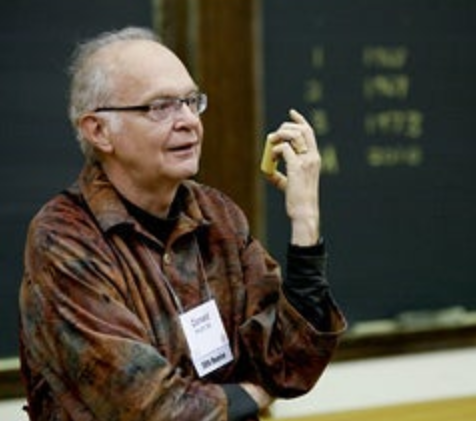
\includegraphics[width=0.7\linewidth]{figs/knuth}
        \end{column}
        
        \begin{column}{0.4\textwidth}
            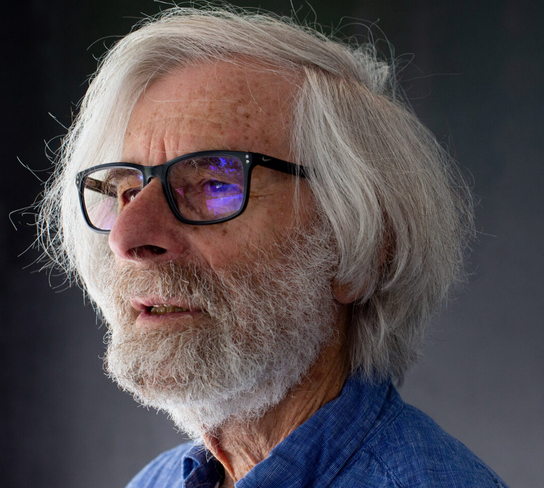
\includegraphics[width=0.9\linewidth]{figs/Lamport}
        \end{column}
    \end{columns}
\end{frame}


\begin{frame}{Latex vs. Word?}
	\begin{columns}
		\begin{column}{0.6\textwidth}
	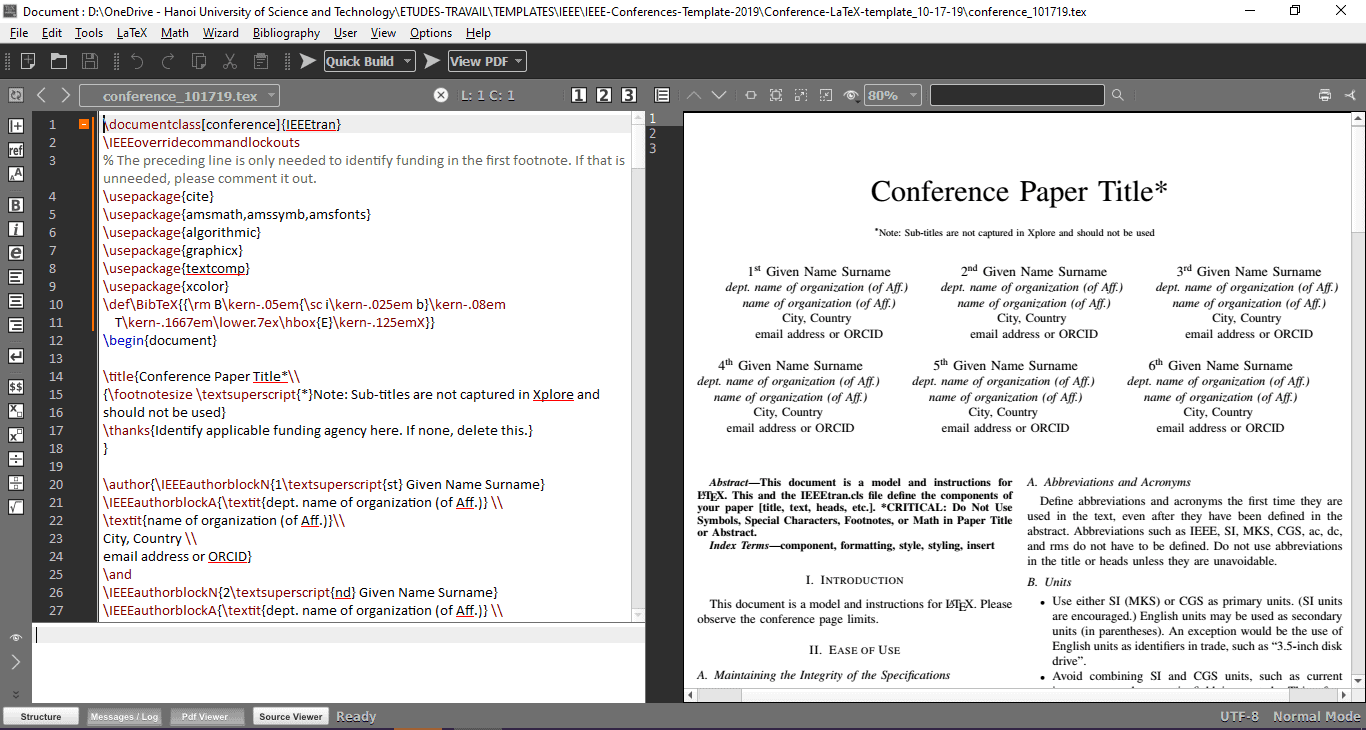
\includegraphics[width=0.9\linewidth]{figs/latex_code}
		\end{column}
		
		\begin{column}{0.4\textwidth}
	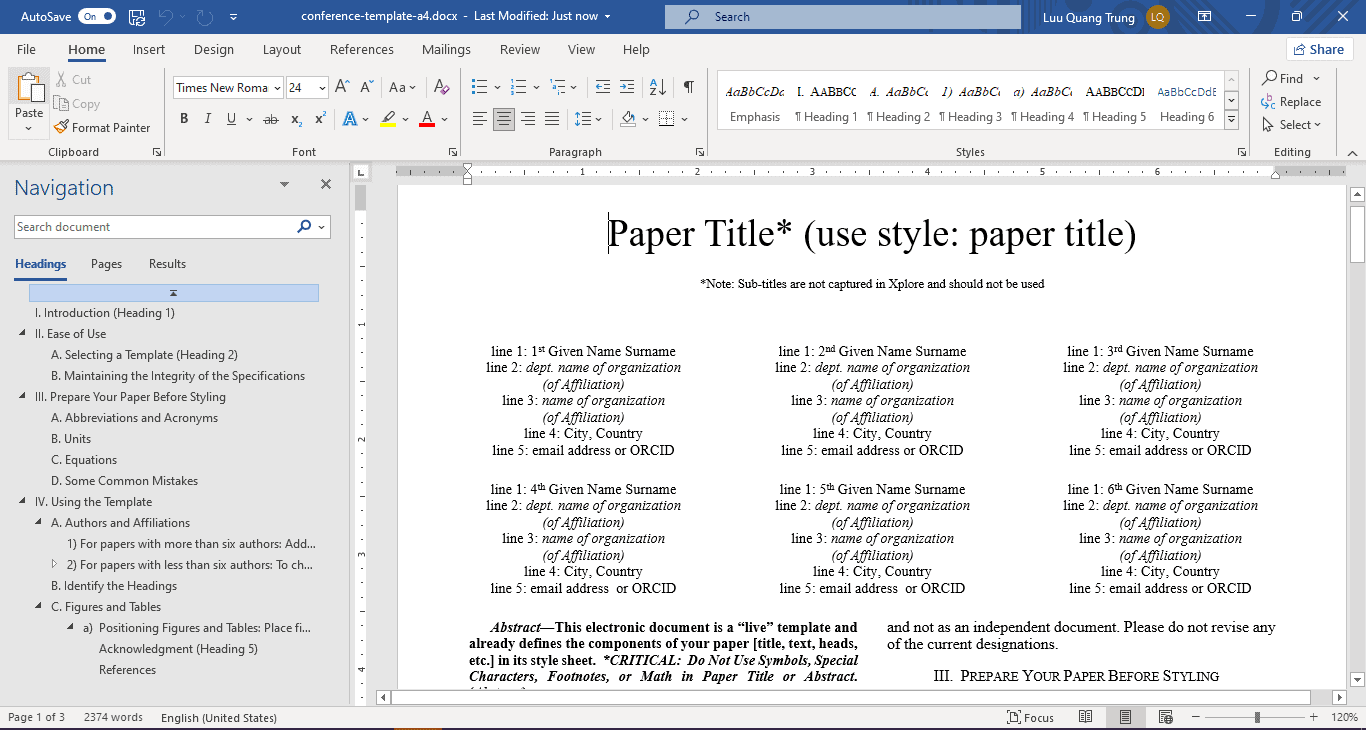
\includegraphics[width=1.0\linewidth]{figs/latex_code1}
		\end{column}
	\end{columns}
\end{frame}


\begin{frame}{Why Use LaTeX?}
    \begin{columns}
        \begin{column}{0.5\textwidth}
            \textbf{Strengths:}
            \begin{itemize}
                \item \alert{Professional typesetting} of mathematics
                \item Consistent formatting throughout documents
                \item Automatic numbering (equations, figures, etc.)
                \item Robust cross-referencing
                \item Bibliography management
                \item Scalable from short notes to books
                \item Stable and free
            \end{itemize}
        \end{column}
        
        \begin{column}{0.5\textwidth}
            %                \includegraphics[width=\textwidth]{example-image-b}
            \begin{center}
                Compare: Word vs. LaTeX output
            \end{center}
            
            \begin{alertblock}{LaTeX shines when:}
                \begin{itemize}
                    \item Documents contain complex mathematics
                    \item Consistency is crucial
                    \item Document will be revised multiple times
                \end{itemize}
            \end{alertblock}
        \end{column}
    \end{columns}
\end{frame}

\begin{frame}{LaTeX Workflow}
    \begin{enumerate}
        \item Write source code (.tex file)
        \item Compile the document
        \item View the output (PDF)
        \item Revise and repeat
    \end{enumerate}
    
    \begin{center}
        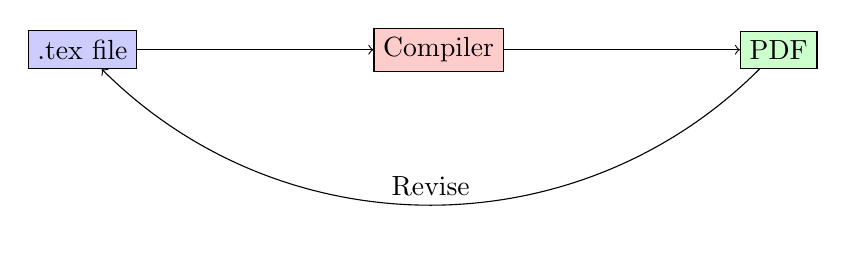
\begin{tikzpicture}[node distance=3cm, auto]
            \usetikzlibrary{positioning} % Add this line to load the positioning library
            \node (source) [rectangle, draw, fill=blue!20] {.tex file};
            \node (compile) [rectangle, draw, fill=red!20, right=of source] {Compiler};
            \node (output) [rectangle, draw, fill=green!20, right=of compile] {PDF};
            \draw[->] (source) -- (compile);
            \draw[->] (compile) -- (output);
            \draw[->] (output) to[bend left=45] node[above] {Revise} (source);
        \end{tikzpicture}
    \end{center}
    
    \begin{tip}
        Most LaTeX editors provide buttons for compile, view, and other common actions
    \end{tip}
\end{frame}

\begin{frame}[fragile]{Your First LaTeX Document}
    \begin{columns}
        \begin{column}{0.5\textwidth}
\begin{lstlisting}
\documentclass{article}

\begin{document}
    Hello, world!
    
    This is my first \LaTeX{} document.
\end{document}
\end{lstlisting}
        \end{column}
        
        \begin{column}{0.5\textwidth}
            \begin{itemize}
                \item Every document starts with \texttt{\textbackslash documentclass}
                \item The actual content goes between:
                \begin{itemize}
                    \item \texttt{\textbackslash begin\{document\}}
                    \item \texttt{\textbackslash end\{document\}}
                \end{itemize}
                \item Commands start with backslash \texttt{\textbackslash}
                \item Some commands take arguments in \{\}
            \end{itemize}
        \end{column}
    \end{columns}
    
    \begin{practice}
        Create this simple document in your editor and compile it
    \end{practice}
\end{frame}

\begin{frame}[fragile]{Document Classes}
    \begin{columns}
        \begin{column}{0.5\textwidth}
            \begin{lstlisting}
\documentclass[12pt,a4paper]{article}
\documentclass{report}
\documentclass{book}
\documentclass{letter}
\documentclass{beamer}
            \end{lstlisting}
        \end{column}
        
        \begin{column}{0.5\textwidth}
            \begin{itemize}
                \item \texttt{article}: Short documents, papers
                \item \texttt{report}: Longer reports with chapters
                \item \texttt{book}: Full books
                \item \texttt{letter}: Correspondence
                \item \texttt{beamer}: Presentations (like this one!)
            \end{itemize}
            
            \textbf{Options in square brackets:}
            \begin{itemize}
                \item Font size: \texttt{10pt}, \texttt{11pt}, \texttt{12pt}
                \item Paper size: \texttt{a4paper}, \texttt{letterpaper}
                \item Columns: \texttt{twocolumn}, \texttt{onecolumn}
                \item And many more...
            \end{itemize}
        \end{column}
    \end{columns}
\end{frame}

\begin{frame}{Comments and Useful Tips in \LaTeX}
	
	\begin{itemize}
		\item \textbf{Comments} in \LaTeX: use the \texttt{\%} symbol
		\begin{itemize}
			\item Example: \texttt{\% This is a comment, it will not appear in the output}
			\item Everything after \texttt{\%} on the same line is ignored.
		\end{itemize}
		\vspace{0.3cm}
		
		\item \textbf{Spacing}: multiple spaces and line breaks are treated as a single space.
%		\begin{itemize}
%			\item To force a new line, use \verb|\\|.
%			\item For more vertical space: \verb|\vspace{length}|.
%		\end{itemize}
		\vspace{0.3cm}
		
		\item \textbf{Special Characters}: some symbols must be escaped.
		\begin{itemize}
			\item Examples: \texttt{\$ \% \_ \{ \} \# \& \textbackslash}.
			\item To print them, use \texttt{\textbackslash} before the character, e.g., \texttt{\textbackslash\%}.
		\end{itemize}
		
		\vspace{0.3cm}
		\item \textbf{Good Practice}: use comments to document your source code.
		\begin{itemize}
			\item Helps collaborators and your future self.
			\item Example: \texttt{\% This section introduces the main theorem.}
		\end{itemize}
%		
	\end{itemize}
	
\end{frame}

\begin{frame}[fragile]{The Preamble and Packages}
    \begin{columns}
        \begin{column}{0.5\textwidth}
            \begin{lstlisting}
\documentclass{article}

% This is the preamble
\usepackage{amsmath}
\usepackage{amssymb}
\usepackage{graphicx}
\usepackage[margin=1in]{geometry}
\usepackage{hyperref}

\title{My Mathematics Document}
\author{Your Name}
\date{\today}

\begin{document}
    \maketitle
    % Document content here...
\end{document}
            \end{lstlisting}
        \end{column}
        
        \begin{column}{0.5\textwidth}
            \begin{itemize}
                \item The \alert{preamble} is everything between the document class and \texttt{\textbackslash begin\{document\}}
                \item \texttt{\textbackslash usepackage} adds functionality
                \item Common packages for mathematics:
                \begin{itemize}
                    \item \texttt{amsmath}: Enhanced math features
                    \item \texttt{amssymb}: Additional math symbols
                    \item \texttt{graphicx}: For including images
                    \item \texttt{geometry}: Page layout control
                    \item \texttt{hyperref}: PDF links and bookmarks
                \end{itemize}
            \end{itemize}
        \end{column}
    \end{columns}
    
    \begin{tip}
        Packages can have options in square brackets: \texttt{\textbackslash usepackage[options]\{package\}}
    \end{tip}
\end{frame}

\begin{frame}[fragile]{Document Structure}
    \begin{columns}
        \begin{column}{0.5\textwidth}
            \begin{lstlisting}
\documentclass{article}
\usepackage{amsmath}

\begin{document}
    \title{Introduction to Calculus}
    \author{Dr. Mathematics}
    \date{June 2025}
    \maketitle
    
    \section{Introduction}
    Calculus is fundamental to...
    
    \section{Derivatives}
    \subsection{Definition}
    The derivative is defined as...
    
    \subsection{Rules}
    Product rule, chain rule...
    
    \section{Conclusion}
\end{document}
            \end{lstlisting}
        \end{column}
        
        \begin{column}{0.5\textwidth}
            \textbf{Sectioning commands:}
            \begin{itemize}
                \item \texttt{\textbackslash section\{Title\}}
                \item \texttt{\textbackslash subsection\{Title\}}
                \item \texttt{\textbackslash subsubsection\{Title\}}
            \end{itemize}
            
            \textbf{For book/report classes:}
            \begin{itemize}
                \item \texttt{\textbackslash chapter\{Title\}} (highest level)
                \item \texttt{\textbackslash part\{Title\}} (even higher)
            \end{itemize}
            
            \textbf{Unnumbered versions:}
            \begin{itemize}
                \item \texttt{\textbackslash section*\{Title\}}
            \end{itemize}
        \end{column}
    \end{columns}
\end{frame}

\begin{frame}[fragile]{Basic Text Formatting}
    \begin{columns}
        \begin{column}{0.5\textwidth}
\begin{lstlisting}
% Font styles
Normal text
\textbf{Bold text}
\textit{Italic text}
\underline{Underlined text}
\texttt{Monospace text}

% Size changes
{\tiny Tiny text} 
{\small Small text}
{\large Large text} 
{\huge Huge text}

% Special characters
\& \% \$ \# \_ \{ \} \~{} \^{} 
\textbackslash

% New paragraph
First paragraph.

Second paragraph.
\end{lstlisting}
        \end{column}
        
        \begin{column}{0.5\textwidth}
            \textbf{Font styles:}
            \begin{itemize}
                \item Normal text
                \item \textbf{Bold text}
                \item \textit{Italic text}
                \item \underline{Underlined text}
                \item \texttt{Monospace text}
            \end{itemize}
            
            \textbf{Size changes:}
            {\tiny Tiny text} {\small Small text} Normal text {\large Large text} {\huge Huge text}
            
            \textbf{Special characters:}
            \& \% \$ \# \_ \{ \} \~{} \^{} \textbackslash
            
            \textbf{New paragraph:} Empty line (not indentation)
        \end{column}
    \end{columns}
\end{frame}

\begin{frame}[fragile]{Lists}
    \begin{columns}
        \begin{column}{0.5\textwidth}
\begin{lstlisting}
% Unordered list (bullet points)
\begin{itemize}
    \item First item
    \item Second item
    \begin{itemize}
        \item Nested item
        \item Another nested item
    \end{itemize}
    \item Third item
\end{itemize}

% Ordered list (numbered)
\begin{enumerate}
    \item First step
    \item Second step
    \begin{enumerate}
        \item Substep A
        \item Substep B
    \end{enumerate}
    \item Third step
\end{enumerate}
\end{lstlisting}
        \end{column}
        
        \begin{column}{0.5\textwidth}
            \textbf{Unordered list:}
            \begin{itemize}
                \item First item
                \item Second item
                \begin{itemize}
                    \item Nested item
                    \item Another nested item
                \end{itemize}
                \item Third item
            \end{itemize}
            
            \textbf{Ordered list:}
            \begin{enumerate}
                \item First step
                \item Second step
                \begin{enumerate}
                    \item Substep A
                    \item Substep B
                \end{enumerate}
                \item Third step
            \end{enumerate}
        \end{column}
    \end{columns}
\end{frame}

\begin{frame}[fragile]{Simple Tables}
    \begin{columns}
        \begin{column}{0.5\textwidth}
            \begin{lstlisting}
\begin{center}
    \begin{tabular}{|l|c|r|}
        \hline
        Left & Center & Right \\
        \hline
        1 & 2 & 3 \\
        4 & 5 & 6 \\
        \hline
    \end{tabular}
\end{center}

% Professional tables with booktabs
\begin{center}
    \begin{tabular}{lcr}
        \toprule
        Left & Center & Right \\
        \midrule
        1 & 2 & 3 \\
        4 & 5 & 6 \\
        \bottomrule
    \end{tabular}
\end{center}
            \end{lstlisting}
        \end{column}
        
        \begin{column}{0.5\textwidth}
            \begin{center}
                \begin{tabular}{|l|c|r|}
                    \hline
                    Left & Center & Right \\
                    \hline
                    1 & 2 & 3 \\
                    4 & 5 & 6 \\
                    \hline
                \end{tabular}
            \end{center}
            
            \textbf{With booktabs package (professional):}
            \begin{center}
                \begin{tabular}{lcr}
                    \toprule
                    Left & Center & Right \\
                    \midrule
                    1 & 2 & 3 \\
                    4 & 5 & 6 \\
                    \bottomrule
                \end{tabular}
            \end{center}
            
            \textbf{Column alignment:}
            \begin{itemize}
                \item \texttt{l} - left align
                \item \texttt{c} - center align
                \item \texttt{r} - right align
                \item \texttt{|} - vertical line
            \end{itemize}
        \end{column}
    \end{columns}
\end{frame}

\begin{frame}{Exercise 1: Basic Document Structure}
    \begin{practice}
        \textbf{Create a 1-page document with:}
        \begin{enumerate}
            \item Title, author, date
            \item Section and subsection headings
            \item A paragraph with bold and italic text
            \item A numbered list and a bullet-point list
            \item A simple table
        \end{enumerate}
    \end{practice}
    
    \begin{tip}
        \begin{itemize}
            \item Start with the basic document structure
            \item Add elements one by one
            \item Compile after adding each element to catch errors quickly
        \end{itemize}
    \end{tip}
\end{frame}


    %------------------------------------------------
    % session 02: MATHEMATICAL TYPESETTING
    %------------------------------------------------
	\section{Mathematical Typesetting}

\begin{frame}[fragile]{Inline vs. Display Math}
    \begin{columns}
        \begin{column}{0.5\textwidth}
            \begin{lstlisting}
% Inline math (within text):
Einstein's equation $E = mc^2$ 
revolutionized physics.

The quadratic formula is 
$x = \frac{-b \pm \sqrt{b^2 - 4ac}}{2a}$.

% Display math (centered, set apart):
\[
E = mc^2
\]

\begin{equation}
    x = \frac{-b \pm \sqrt{b^2 - 4ac}}{2a}
\end{equation}
            \end{lstlisting}
        \end{column}
        
        \begin{column}{0.5\textwidth}
            \textbf{Inline math:}
            \begin{itemize}
                \item Inside text flow: $E = mc^2$
                \item Uses \texttt{\$...\$} or \texttt{\textbackslash(..\\textbackslash)} delimiters
                \item Less vertical space
                \item Avoids line breaks
            \end{itemize}
            
            \textbf{Display math:}
            \begin{itemize}
                \item Set apart from text
                \item Centered on its own line
                \item \texttt{\textbackslash[...\textbackslash]} (unnumbered)
                \item \texttt{equation} environment (numbered)
            \end{itemize}
        \end{column}
    \end{columns}
    
    \begin{warning}
        Never use \texttt{\$\$...\$\$} for display math in LaTeX (a TeX relic)
    \end{warning}
\end{frame}

\begin{frame}[fragile]{Basic Math Syntax}
    \begin{columns}
        \begin{column}{0.5\textwidth}
            \begin{lstlisting}
% Subscripts and superscripts
$x^2$         % superscript
$x_i$         % subscript
$x_i^2$       % both
$x^{2n}$      % multi-character
$x_{i,j}$     % multi-character
$x^2_i$       % both

% Fractions
$\frac{1}{2}$           % standard
$\frac{\partial f}{\partial x}$  % complex
$\tfrac{1}{2}$          % text-style

% Square roots
$\sqrt{x}$              % square root
$\sqrt[3]{x}$           % cube root
            \end{lstlisting}
        \end{column}
        
        \begin{column}{0.5\textwidth}
            \textbf{Subscripts and superscripts:}
            \begin{itemize}
                \item $x^2$ (superscript)
                \item $x_i$ (subscript)
                \item $x_i^2$ (both)
                \item $x^{2n}$ (multi-character superscript)
                \item $x_{i,j}$ (multi-character subscript)
            \end{itemize}
            
            \textbf{Fractions:}
            \begin{itemize}
                \item $\frac{1}{2}$ (standard)
                \item $\frac{\partial f}{\partial x}$ (complex)
                \item $\tfrac{1}{2}$ (text-style)
            \end{itemize}
            
            \textbf{Square roots:}
            \begin{itemize}
                \item $\sqrt{x}$ (square root)
                \item $\sqrt[3]{x}$ (cube root)
            \end{itemize}
        \end{column}
    \end{columns}
\end{frame}

\begin{frame}[fragile]{Greek Letters and Special Symbols}
    \begin{columns}
        \begin{column}{0.5\textwidth}
            \begin{lstlisting}
% Lowercase Greek letters
$\alpha, \beta, \gamma, \delta$
$\epsilon, \varepsilon, \zeta, \eta$
$\theta, \vartheta, \iota, \kappa$
$\lambda, \mu, \nu, \xi$
$o, \pi, \varpi, \rho, \varrho$
$\sigma, \varsigma, \tau, \upsilon$
$\phi, \varphi, \chi, \psi, \omega$

% Uppercase Greek letters
$\Gamma, \Delta, \Theta, \Lambda$
$\Xi, \Pi, \Sigma, \Upsilon$
$\Phi, \Psi, \Omega$

% Special symbols
$\infty, \partial, \nabla, \wp$
$\emptyset, \forall, \exists$
$\in, \notin, \subset, \supset$
$\cup, \cap, \setminus$
            \end{lstlisting}
        \end{column}
        
        \begin{column}{0.5\textwidth}
            \textbf{Lowercase Greek:}
            \begin{center}
$\alpha, \beta, \gamma, \delta$\\
$\epsilon, \varepsilon, \zeta, \eta$\\
$\theta, \vartheta, \iota, \kappa$\\
$\lambda, \mu, \nu, \xi$\\
$o, \pi, \varpi, \rho, \varrho$\\
$\sigma, \varsigma, \tau, \upsilon$\\
$\phi, \varphi, \chi, \psi, \omega$
            \end{center}
            
            \textbf{Uppercase Greek:}
            \begin{center}
$\Gamma, \Delta, \Theta, \Lambda$\\
$\Xi, \Pi, \Sigma, \Upsilon$\\
$\Phi, \Psi, \Omega$
            \end{center}
            
            \textbf{Special symbols:}
            \begin{center}
$\infty, \partial, \nabla, \wp$\\
$\emptyset, \forall, \exists$\\
$\in, \notin, \subset, \supset$\\
$\cup, \cap, \setminus$
            \end{center}
        \end{column}
    \end{columns}
\end{frame}

\begin{frame}[fragile]{Mathematical Operators and Relations}
    \begin{columns}
        \begin{column}{0.5\textwidth}
\begin{lstlisting}
% Binary relations
$=, \ne, \approx, \sim, \cong$
$<, \le, >, \ge$
$\ll, \gg, \prec, \succ$

% Binary operators
$+, -, \times, \div, \pm, \mp$
$\cdot, \ast, \star, \circ, \bullet$
$\cup, \cap, \setminus, \wedge, \vee$

% Large operators
$\sum_{i=1}^{n} i = \frac{n(n+1)}{2}$

$\prod_{i=1}^{n} i = n!$

$\int_{a}^{b} f(x) \, dx$

$\oint_C f(z) \, dz = 2\pi i$

$\lim_{x \to 0} \frac{\sin x}{x} = 1$
\end{lstlisting}
        \end{column}
        
        \begin{column}{0.5\textwidth}
            \textbf{Binary relations:}
            \begin{center}
                $=, \ne, \approx, \sim, \cong$\\
                $<, \le, >, \ge$\\
                $\ll, \gg, \prec, \succ$
            \end{center}
            
            \textbf{Binary operators:}
            \begin{center}
                $+, -, \times, \div, \pm, \mp$\\
                $\cdot, \ast, \star, \circ, \bullet$\\
                $\cup, \cap, \setminus, \wedge, \vee$
            \end{center}
            
            \textbf{Large operators:}
            \begin{align*}
                \sum_{i=1}^{n} i &= \frac{n(n+1)}{2}\\
                \prod_{i=1}^{n} i &= n!\\
                \int_{a}^{b} f(x) \, dx\\
                \oint_C f(z) \, dz &= 2\pi i\\
                \lim_{x \to 0} \frac{\sin x}{x} &= 1
            \end{align*}
        \end{column}
    \end{columns}
\end{frame}

\begin{frame}[fragile]{Function Names}
    \begin{columns}
        \begin{column}{0.5\textwidth}
            \begin{lstlisting}
% Wrong way (italicized)
$sin(x)$
$log(x)$
$lim_{x \to 0} f(x)$

% Correct way (upright)
$\sin(x)$
$\log(x)$
$\lim_{x \to 0} f(x)$
                
                % Common function names
$\sin(x), \cos(x), \tan(x)$
$\arcsin(x), \arccos(x), \arctan(x)$
$\exp(x), \ln(x), \log_{10}(x)$
$\min(x,y), \max(x,y)$
$\gcd(a,b), \det(A), \dim(V)$
            \end{lstlisting}
        \end{column}
        
        \begin{column}{0.5\textwidth}
            \textbf{Wrong (italicized):}
            \begin{itemize}
                \item $sin(x)$
                \item $log(x)$
                \item $lim_{x \to 0} f(x)$
            \end{itemize}
            
            \textbf{Correct (upright):}
            \begin{itemize}
                \item $\sin(x)$
                \item $\log(x)$
                \item $\lim_{x \to 0} f(x)$
            \end{itemize}
            
            \textbf{Common function names:}
            \begin{itemize}
                \item $\sin(x), \cos(x), \tan(x)$
                \item $\arcsin(x), \arccos(x), \arctan(x)$
                \item $\exp(x), \ln(x), \log_{10}(x)$
                \item $\min(x,y), \max(x,y)$
                \item $\gcd(a,b), \det(A), \dim(V)$
            \end{itemize}
        \end{column}
    \end{columns}
    
    \begin{tip}
        Always use the backslash command for function names
    \end{tip}
\end{frame}

\begin{frame}[fragile]{Delimiters (Brackets and Parentheses)}
    \begin{columns}
        \begin{column}{0.5\textwidth}
\begin{lstlisting}
% Fixed size
$(x)$
$[x]$
$\{x\}$
$|x|$
$\|x\|$
$\langle x \rangle$
$\lceil x \rceil$
$\lfloor x \rfloor$

% Auto-scaling
$\left( \frac{1}{1-x^2} \right)$

$\left[ \sum_{i=1}^{n} a_i \right]$

$\left\{ \frac{n(n+1)}{2} \right\}$

$\left| \det(A) \right|$
\end{lstlisting}
        \end{column}
        
        \begin{column}{0.5\textwidth}
            \textbf{Fixed size:}
            \begin{center}
                $(x)$ - parentheses\\
                $[x]$ - square brackets\\
                $\{x\}$ - curly braces\\
                $|x|$ - absolute value\\
                $\|x\|$ - norm\\
                $\langle x \rangle$ - angle brackets\\
                $\lceil x \rceil$ - ceiling\\
                $\lfloor x \rfloor$ - floor
            \end{center}
            
            \textbf{Auto-scaling:}
            \begin{center}
                $\left( \frac{1}{1-x^2} \right)$\\[5pt]
                $\left[ \sum_{i=1}^{n} a_i \right]$\\[5pt]
                $\left\{ \frac{n(n+1)}{2} \right\}$\\[5pt]
                $\left| \det(A) \right|$
            \end{center}
        \end{column}
    \end{columns}
    
    \begin{tip}
        Always use \texttt{\textbackslash left} and \texttt{\textbackslash right} for complex expressions
    \end{tip}
\end{frame}

\begin{frame}[fragile]{Matrices}
    \begin{columns}
        \begin{column}{0.5\textwidth}
\begin{lstlisting}
    % Matrix without delimiters
    \begin{matrix}
        a & b \\
        c & d
    \end{matrix}
    
    % Matrix with parentheses
    \begin{pmatrix}
        a & b \\
        c & d
    \end{pmatrix}
    
    % Matrix with brackets
    \begin{bmatrix}
        a & b \\
        c & d
    \end{bmatrix}
    
    % Matrix with braces
    \begin{Bmatrix}
        a & b \\
        c & d
    \end{Bmatrix}
    
    % Matrix with vertical bars
    \begin{vmatrix}
        a & b \\
        c & d
    \end{vmatrix}
\end{lstlisting}
        \end{column}
        
        \begin{column}{0.5\textwidth}
            \begin{center}
                $\begin{matrix} a & b \\ c & d \end{matrix}$ - no delimiters\\[10pt]
                
                $\begin{pmatrix} a & b \\ c & d \end{pmatrix}$ - parentheses\\[10pt]
                
                $\begin{bmatrix} a & b \\ c & d \end{bmatrix}$ - brackets\\[10pt]
                
                $\begin{Bmatrix} a & b \\ c & d \end{Bmatrix}$ - braces\\[10pt]
                
                $\begin{vmatrix} a & b \\ c & d \end{vmatrix}$ - determinant
            \end{center}
            
            \begin{itemize}
                \item Use \texttt{\&} to separate columns
                \item Use \texttt{\\} for new rows
                \item Requires \texttt{amsmath} package
            \end{itemize}
        \end{column}
    \end{columns}
\end{frame}

\begin{frame}[fragile]{Equation Alignment}
    \begin{columns}
        \begin{column}{0.5\textwidth}
            \begin{lstlisting}
% Multiple equations (numbered)
\begin{align}
    E &= mc^2 \\
    F &= ma
\end{align}

% Multiple equations (unnumbered)
\begin{align*}
    (a+b)^2 &= (a+b)(a+b) \\
    &= a(a+b) + b(a+b) \\
    &= a^2 + ab + ba + b^2 \\
    &= a^2 + 2ab + b^2
\end{align*}

% Align at multiple places
\begin{align}
    f(x) &= (x+a)(x+b) \\
    &= x^2 + (a+b)x + ab \\
    &= x^2 + cx + d
\end{align}
            \end{lstlisting}
        \end{column}
        
        \begin{column}{0.5\textwidth}
            \textbf{Multiple equations (numbered):}
            \begin{align}
                E &= mc^2 \\
                F &= ma
            \end{align}
            
            \textbf{Multiple equations (unnumbered):}
            \begin{align*}
                (a+b)^2 &= (a+b)(a+b) \\
                &= a(a+b) + b(a+b) \\
                &= a^2 + ab + ba + b^2 \\
                &= a^2 + 2ab + b^2
            \end{align*}
            
            \begin{itemize}
                \item Alignment point is marked with \texttt{\&}
                \item Each line ends with \texttt{\\}
                \item \texttt{align*} for unnumbered equations
                \item Requires \texttt{amsmath} package
            \end{itemize}
        \end{column}
    \end{columns}
    
    \begin{tip}
        Always align equations at the relation symbol (=, <, etc.)
    \end{tip}
\end{frame}

\begin{frame}[fragile]{Cases and Multi-Line Expressions}
    \begin{columns}
        \begin{column}{0.5\textwidth}
            \begin{lstlisting}
                % Cases (piecewise functions)
                \begin{equation}
                    |x| = 
                    \begin{cases}
                        x & \text{if } x \geq 0 \\
                        -x & \text{if } x < 0
                    \end{cases}
                \end{equation}
                
                % Multi-line expression
                \begin{equation}
                    \begin{split}
                        (a+b)^3 = &(a+b)^2(a+b) \\
                        = &(a^2+2ab+b^2)(a+b) \\
                        = &a^3 + 2a^2b + ab^2 \\
                        &+ a^2b + 2ab^2 + b^3 \\
                        = &a^3 + 3a^2b + 3ab^2 + b^3
                    \end{split}
                \end{equation}
            \end{lstlisting}
        \end{column}
        
        \begin{column}{0.5\textwidth}
            \textbf{Cases (piecewise functions):}
            \begin{equation}
                |x| = 
                \begin{cases}
                    x & \text{if } x \geq 0 \\
                    -x & \text{if } x < 0
                \end{cases}
            \end{equation}
            
            \textbf{Multi-line expression:}
            \begin{equation}
                \begin{split}
                    (a+b)^3 = &(a+b)^2(a+b) \\
                    = &(a^2+2ab+b^2)(a+b) \\
                    = &a^3 + 2a^2b + ab^2 \\
                    &+ a^2b + 2ab^2 + b^3 \\
                    = &a^3 + 3a^2b + 3ab^2 + b^3
                \end{split}
            \end{equation}
            
            \begin{tip}
                Use \texttt{\textbackslash text\{...\}} for text within math mode
            \end{tip}
        \end{column}
    \end{columns}
\end{frame}

\begin{frame}[fragile]{Additional Math Environments}
    \begin{columns}
        \begin{column}{0.5\textwidth}
            \begin{lstlisting}
% Gather - centered, multi-line
\begin{gather}
    a_1 = b_1 + c_1\\
    a_2 = b_2 + c_2 + d_2
\end{gather}

% Numbered array
\begin{array}{lcr}
    left & center & right\\
    x+y & x & y
\end{array}

% Multiline equation
\begin{multline}
    a + b + c + d + e + f \\
    + i + j + k + l + m
\end{multline}

% Subequations (hierarchical numbering)
\begin{subequations}
    \begin{align}
        a &= b + c\\
        d &= e + f
    \end{align}
\end{subequations}
            \end{lstlisting}
        \end{column}
        
        \begin{column}{0.5\textwidth}
            \textbf{Gather} - centered equations:
            \begin{gather}
                a_1 = b_1 + c_1\\
                a_2 = b_2 + c_2 + d_2
            \end{gather}
            
            \textbf{Array} - tabular math:
            \begin{center}
                $\begin{array}{lcr}
                    \text{left} & \text{center} & \text{right}\\
                    x+y & x & y
                \end{array}$
            \end{center}
            
            \textbf{Multline} - break long equations:
            \begin{multline}
                a + b + c + d + e + f \\
                + i + j + k + l + m
            \end{multline}
            
            \textbf{Subequations} - hierarchical:
            \begin{subequations}
                \begin{align}
                    a &= b + c\\
                    d &= e + f
                \end{align}
            \end{subequations}
        \end{column}
    \end{columns}
\end{frame}

\begin{frame}{Exercise 2: Mathematical Typesetting}
    \begin{practice}
        \textbf{Create a document with these mathematical elements:}
        \begin{enumerate}
            \item A paragraph with inline math expressions
            \item Multiple display math equations (both numbered and unnumbered)
            \item An equation with fractions, superscripts, subscripts, and Greek letters
            \item A piecewise function using cases
            \item A matrix equation
            \item A multi-line derivation with proper alignment
        \end{enumerate}
    \end{practice}
    
    \begin{tip}
        \begin{itemize}
            \item Use \texttt{align} for multiple aligned equations
            \item Remember \texttt{\textbackslash left} and \texttt{\textbackslash right} for auto-scaling delimiters
            \item Test complex expressions separately before combining them
        \end{itemize}
    \end{tip}
\end{frame}


	%------------------------------------------------
	% session 03: DOCUMENT STRUCTURE
	%------------------------------------------------

	
\section{Structuring a Mathematical Document}

\begin{frame}[fragile]{Theorems and Mathematical Environments - Basics}
	\begin{columns}
		\begin{column}{0.5\textwidth}
			\begin{lstlisting}[basicstyle=\footnotesize\ttfamily]
				% In preamble
				\usepackage{amsthm}
				
				% Define theorem-like environments
				\newtheorem{theorem}{Theorem}[section]
				\newtheorem{lemma}[theorem]{Lemma}
				\newtheorem{proposition}[theorem]{Proposition}
				\newtheorem{corollary}[theorem]{Corollary}
				
				\theoremstyle{definition}
				\newtheorem{definition}[theorem]{Definition}
				\newtheorem{example}[theorem]{Example}
				
				\theoremstyle{remark}
				\newtheorem{remark}[theorem]{Remark}
				\newtheorem{note}[theorem]{Note}
			\end{lstlisting}
		\end{column}
		
		\begin{column}{0.5\textwidth}
			\textbf{Theorem-like environments:}
			\begin{itemize}
				\item Theorem, lemma, proposition, corollary
				\item Definition, example
				\item Remark, note
			\end{itemize}
			
			\textbf{Theorem styles:}
			\begin{itemize}
				\item \texttt{plain} (default): Bold title, italic body
				\item \texttt{definition}: Bold title, roman body
				\item \texttt{remark}: Italic title, roman body
			\end{itemize}
			
			\textbf{Numbering options:}
			\begin{itemize}
				\item \texttt{[section]} - restart in each section
				\item \texttt{[theorem]} - share counters
			\end{itemize}
		\end{column}
	\end{columns}
	
	\begin{tip}
		Define theorem environments in the preamble to use throughout your document
	\end{tip}
\end{frame}

\begin{frame}[fragile]{Using Theorems and Proofs}
	\begin{columns}
		\begin{column}{0.5\textwidth}
			\begin{lstlisting}[basicstyle=\footnotesize\ttfamily]
				% Basic usage
				\begin{theorem}[Pythagorean Theorem]
					In a right triangle, the square of the 
					hypotenuse equals the sum of squares 
					of the other two sides.
				\end{theorem}
				
				\begin{proof}
					This follows from... [proof details]
				\end{proof}
				
				% Famous example
				\begin{theorem}[Fermat's Last Theorem]
					If $n > 2$ is a positive integer, then 
					the equation
					\[
					a^n + b^n = c^n
					\]
					has no solutions in positive integers 
					$a$, $b$, and $c$.
				\end{theorem}
			\end{lstlisting}
		\end{column}
		
		\begin{column}{0.5\textwidth}
			\def\labelenumi{\Roman{enumi}.}
			
			\begin{block}{Rendered output:}
				\textbf{Theorem 1} (Pythagorean Theorem). \textit{In a right triangle, the square of the hypotenuse equals the sum of squares of the other two sides.}
				
				\textit{Proof.} This follows from... [proof details] \hfill $\square$
				
				\vspace{1em}
				
				\textbf{Theorem 2} (Fermat's Last Theorem). \textit{If $n > 2$ is a positive integer, then the equation
					\[
					a^n + b^n = c^n
					\]
					has no solutions in positive integers $a$, $b$, and $c$.}
			\end{block}
			
			\textbf{Special features:}
			\begin{itemize}
				\item Optional theorem name in []
				\item \texttt{proof} environment adds QED symbol ($\square$)
				\item Can include math displays inside theorems
			\end{itemize}
		\end{column}
	\end{columns}
	
	\begin{tip}
		For papers, check if the target journal provides specific theorem definitions
	\end{tip}
\end{frame}

\begin{frame}[fragile]{Definition and Example Environments}
	\begin{columns}
		\begin{column}{0.5\textwidth}
			\begin{lstlisting}[basicstyle=\footnotesize\ttfamily]
				\begin{definition}[Continuous Function]
					A function $f$ is continuous at point $a$
					if $\lim_{x \to a} f(x) = f(a)$.
				\end{definition}
				
				\begin{example}
					The function $f(x) = x^2$ is continuous
					everywhere.
				\end{example}
				
				\begin{remark}
					Not every function is continuous.
					For instance, $f(x) = 1/x$ is not 
					continuous at $x = 0$.
				\end{remark}
			\end{lstlisting}
		\end{column}
		
		\begin{column}{0.5\textwidth}
			\begin{block}{Rendered output:}
				\textbf{Definition 1} (Continuous Function). A function $f$ is continuous at point $a$ if $\lim_{x \to a} f(x) = f(a)$.
				
				\textbf{Example 2.} The function $f(x) = x^2$ is continuous everywhere.
				
				\textit{Remark 3.} Not every function is continuous. For instance, $f(x) = 1/x$ is not continuous at $x = 0$.
			\end{block}
			
			\textbf{Using multiple theorem types:}
			\begin{itemize}
				\item All share the same counter by default when using \texttt{[theorem]}
				\item Can be referenced with \texttt{\textbackslash ref\{label\}}
				\item Different visual styles help readers identify content types
			\end{itemize}
		\end{column}
	\end{columns}
	
	\begin{tip}
		Consistent use of environments improves document readability and navigation
	\end{tip}
\end{frame}

\begin{frame}[fragile]{Including Graphics}
	\begin{columns}
		\begin{column}{0.5\textwidth}
			\begin{lstlisting}
				% In preamble
				\usepackage{graphicx}
				
				% Basic inclusion
				\begin{figure}
					\centering
					\includegraphics{image-filename}
					\caption{A description of the figure}
					\label{fig:mylabel}
				\end{figure}
				
				% With options
				\begin{figure}
					\centering
					\includegraphics[
					width=0.8\textwidth,
					height=6cm,
					keepaspectratio
					]{image-filename}
					\caption{A description of the figure}
					\label{fig:mylabel}
				\end{figure}
				
				% Reference the figure
				As shown in Figure~\ref{fig:mylabel}...
			\end{lstlisting}
		\end{column}
		
		\begin{column}{0.5\textwidth}
			\textbf{Supported formats:}
			\begin{itemize}
				\item PDF, PNG, JPG (with pdfLaTeX)
				\item PDF, EPS (with LaTeX)
			\end{itemize}
			
			\textbf{Common options:}
			\begin{itemize}
				\item \texttt{width=0.8\textbackslash textwidth}
				\item \texttt{height=6cm}
				\item \texttt{scale=0.5}
				\item \texttt{angle=90}
				\item \texttt{keepaspectratio} (prevents distortion)
			\end{itemize}
			
			\textbf{Figure placement:}
			\begin{itemize}
				\item \texttt{h} - here
				\item \texttt{t} - top
				\item \texttt{b} - bottom
				\item \texttt{p} - separate page
				\item \texttt{!} - override defaults
				\item Example: \texttt{\textbackslash begin\{figure\}[htbp]}
			\end{itemize}
		\end{column}
	\end{columns}
	
	\begin{warning}
		LaTeX decides where to place figures - they may "float" away from where they appear in the source
	\end{warning}
\end{frame}

\begin{frame}[fragile]{Tables as Floats}
	\begin{columns}
		\begin{column}{0.5\textwidth}
			\begin{lstlisting}
				% Professional table with caption
				\begin{table}
					\centering
					\caption{Comparison of algorithms}
					\label{tab:comparison}
					\begin{tabular}{lcc}
						\toprule
						Algorithm & Time & Space \\
						\midrule
						Quicksort & $O(n \log n)$ & $O(n)$ \\
						Mergesort & $O(n \log n)$ & $O(n)$ \\
						Heapsort & $O(n \log n)$ & $O(1)$ \\
						\bottomrule
					\end{tabular}
				\end{table}
				
				% Reference the table
				Table~\ref{tab:comparison} shows...
				
				% Multi-column table
				\begin{tabular}{|c|c|c|}
					\hline
					\multicolumn{2}{|c|}{Combined} & Separate \\
					\hline
					A & B & C \\
					\hline
				\end{tabular}
			\end{lstlisting}
		\end{column}
		
		\begin{column}{0.5\textwidth}
			\textbf{Table vs Tabular:}
			\begin{itemize}
				\item \texttt{table} - float environment (like figure)
				\item \texttt{tabular} - actual content structure
			\end{itemize}
			
			\textbf{Professional tables:}
			\begin{itemize}
				\item Use \texttt{booktabs} package
				\item \texttt{\textbackslash toprule}, \texttt{\textbackslash midrule}, \texttt{\textbackslash bottomrule}
				\item Avoid vertical lines (typographic best practice)
			\end{itemize}
			
			\textbf{Advanced features:}
			\begin{itemize}
				\item \texttt{\textbackslash multicolumn\{2\}\{c\}\{Combined\}}
				\item \texttt{\textbackslash multirow} (requires package)
				\item \texttt{\textbackslash cline\{2-3\}} (partial horizontal line)
				\item \texttt{p\{width\}} column type for paragraph text
			\end{itemize}
		\end{column}
	\end{columns}
	
	\begin{tip}
		Always put tables in \texttt{table} environments with captions and labels
	\end{tip}
\end{frame}

\begin{frame}[fragile]{Cross-Referencing}
	\begin{columns}
		\begin{column}{0.5\textwidth}
			\begin{lstlisting}
				% Labels and references
				\section{Introduction}
				\label{sec:intro}
				
				In Section~\ref{sec:methods}, we...
				
				\begin{equation}
					E = mc^2
					\label{eq:einstein}
				\end{equation}
				
				Equation~\eqref{eq:einstein} shows...
				
				\begin{figure}
					\centering
					\includegraphics{graph}
					\caption{Important data}
					\label{fig:data}
				\end{figure}
				
				As shown in Figure~\ref{fig:data}...
				
				\begin{theorem}
					\label{thm:pythagoras}
					In a right triangle...
				\end{theorem}
				
				By Theorem~\ref{thm:pythagoras}...
			\end{lstlisting}
		\end{column}
		
		\begin{column}{0.5\textwidth}
			\textbf{Labeling conventions:}
			\begin{itemize}
				\item Use prefixes: \texttt{sec:}, \texttt{eq:}, \texttt{fig:}, \texttt{tab:}, \texttt{thm:}
				\item Choose descriptive names
			\end{itemize}
			
			\textbf{Reference commands:}
			\begin{itemize}
				\item \texttt{\textbackslash ref\{label\}} - general reference
				\item \texttt{\textbackslash eqref\{label\}} - equation reference (adds parentheses)
				\item \texttt{\textbackslash pageref\{label\}} - page number
			\end{itemize}
			
			\textbf{Tips:}
			\begin{itemize}
				\item Use \texttt{\textasciitilde} for non-breaking space
				\item Run LaTeX twice to resolve references
				\item Use descriptive text: "Theorem~\ref{thm:main}" not just "see~\ref{thm:main}"
			\end{itemize}
		\end{column}
	\end{columns}
	
	\begin{warning}
		If you see "??" in your PDF, you need to compile again
	\end{warning}
\end{frame}

\begin{frame}[fragile]{Table of Contents and Document Divisions}
	\begin{columns}
		\begin{column}{0.5\textwidth}
			\begin{lstlisting}
				\documentclass{article}
				
				\title{Complete Analysis}
				\author{Author Name}
				\date{\today}
				
				\begin{document}
					
					\maketitle
					\tableofcontents
					\listoffigures
					\listoftables
					
					\section{Introduction}
					...
					
					\appendix
					\section{Derivation Details}
					...
					
				\end{document}
			\end{lstlisting}
		\end{column}
		
		\begin{column}{0.5\textwidth}
			\textbf{Automatic lists:}
			\begin{itemize}
				\item \texttt{\textbackslash tableofcontents}
				\item \texttt{\textbackslash listoffigures}
				\item \texttt{\textbackslash listoftables}
			\end{itemize}
			
			\textbf{Document divisions:}
			\begin{itemize}
				\item Front matter: title page, TOC, etc.
				\item Main matter: the content
				\item Back matter: bibliography, appendices
			\end{itemize}
			
			\textbf{Special commands:}
			\begin{itemize}
				\item \texttt{\textbackslash appendix} - changes numbering to A, B, ...
				\item \texttt{\textbackslash part} - for very large documents
			\end{itemize}
			
			\begin{tip}
				Run LaTeX twice to generate proper TOC
			\end{tip}
		\end{column}
	\end{columns}
\end{frame}

\begin{frame}{Exercise 3: Document Structure}
	\begin{practice}
		\textbf{Create a structured mathematical document with:}
		\begin{enumerate}
			\item At least one theorem, definition, and example
			\item A figure with caption and label 
			\item A table with caption and label
			\item Proper cross-references to all elements
			\item A table of contents
			\item At least two sections with mathematical content
		\end{enumerate}
	\end{practice}
	
	\begin{warning}
		Remember to run LaTeX multiple times to resolve references and TOC!
	\end{warning}
	
	\begin{tip}
		Organize your document into logical sections before adding detailed content
	\end{tip}
\end{frame}

	%------------------------------------------------
	% session 4: ADVANCED TOPICS
	%------------------------------------------------
    
\section{Final Tips \& Advanced Topics}

\begin{frame}[fragile]{Bibliography Basics}
	\begin{columns}
		\begin{column}{0.5\textwidth}
			\begin{lstlisting}
				% Manual bibliography
				\begin{thebibliography}{9}
					
					\bibitem{lamport94}
					Leslie Lamport,
					\emph{\LaTeX: A Document Preparation System}.
					Addison Wesley, Massachusetts,
					2nd Edition,
					1994.
					
					\bibitem{knuth84}
					Donald E. Knuth,
					\emph{The \TeX book}.
					Addison Wesley, Massachusetts,
					1984.
					
				\end{thebibliography}
				
				% In-text citation
				According to Lamport~\cite{lamport94},
				\LaTeX{} is...
			\end{lstlisting}
		\end{column}
		
		\begin{column}{0.5\textwidth}
			\textbf{Manual bibliography:}
			\begin{itemize}
				\item \texttt{thebibliography} environment
				\item \texttt{\{9\}} - width hint (number of entries)
				\item \texttt{\textbackslash bibitem\{key\}} - define reference
				\item \texttt{\textbackslash cite\{key\}} - cite reference
			\end{itemize}
			
			\textbf{Limitations:}
			\begin{itemize}
				\item Manual formatting
				\item No automatic sorting
				\item Difficult to maintain
			\end{itemize}
			
			\begin{alertblock}{Brief introduction to BibTeX/BibLaTeX:}
				\begin{itemize}
					\item Separate .bib file with references
					\item Automatic formatting and sorting
					\item More powerful and easier for large bibliographies
					\item Covered in advanced workshops
				\end{itemize}
			\end{alertblock}
		\end{column}
	\end{columns}
\end{frame}

\begin{frame}[fragile]{Introduction to BibTeX}
	\begin{columns}
		\begin{column}{0.5\textwidth}
			\begin{lstlisting}
				% In yourfile.tex
				\documentclass{article}
				\begin{document}
					
					According to Lamport~\cite{lamport94},
					\LaTeX{} is...
					
					\bibliographystyle{plain}
					\bibliography{mybibfile}
					
				\end{document}
			\end{lstlisting}
			
			\begin{lstlisting}
				% In mybibfile.bib
				@book{lamport94,
					author    = {Leslie Lamport},
					title     = {\LaTeX: A Document 
						Preparation System},
					publisher = {Addison Wesley},
					year      = {1994},
					edition   = {2nd},
					address   = {Massachusetts}
				}
				
				@book{knuth84,
					author    = {Donald E. Knuth},
					title     = {The \TeX book},
					publisher = {Addison Wesley},
					year      = {1984},
					address   = {Massachusetts}
				}
			\end{lstlisting}
		\end{column}
		
		\begin{column}{0.5\textwidth}
			\textbf{BibTeX workflow:}
			\begin{enumerate}
				\item Create .bib file with references
				\item \texttt{\textbackslash cite\{key\}} in document
				\item Choose bibliography style
				\item Run: latex → bibtex → latex → latex
			\end{enumerate}
			
			\textbf{Common entry types:}
			\begin{itemize}
				\item \texttt{@article} - journal article
				\item \texttt{@book} - book
				\item \texttt{@incollection} - book chapter
				\item \texttt{@inproceedings} - conference paper
				\item \texttt{@misc} - miscellaneous
			\end{itemize}
			
			\textbf{Common bibliography styles:}
			\begin{itemize}
				\item \texttt{plain} - sorted by author, then year
				\item \texttt{alpha} - [Lam94] style labels
				\item \texttt{unsrt} - citation order
				\item \texttt{abbrv} - abbreviated first names
			\end{itemize}
		\end{column}
	\end{columns}
\end{frame}

\begin{frame}[fragile]{Useful Packages for Mathematicians}
	\begin{columns}
		\begin{column}{0.5\textwidth}
			\textbf{Essential packages:}
			\begin{itemize}
				\item \texttt{amsmath}, \texttt{amssymb} - math typesetting
				\item \texttt{amsthm} - theorems and proofs
				\item \texttt{mathtools} - extends amsmath
				\item \texttt{booktabs} - professional tables
				\item \texttt{graphicx} - for figures
				\item \texttt{hyperref} - links and bookmarks
			\end{itemize}
		\end{column}
		
		\begin{column}{0.5\textwidth}
			\textbf{Additional useful packages:}
			\begin{itemize}
				\item \texttt{tikz}/\texttt{pgfplots} - for creating figures
				\item \texttt{cleveref} - smart references
				\item \texttt{siunitx} - for units and numbers
				\item \texttt{algorithm2e}/\texttt{algorithmicx} - for algorithms
				\item \texttt{tcolorbox} - advanced text boxes
				\item \texttt{microtype} - typographic enhancements
				\item \texttt{todonotes} - comments and notes
			\end{itemize}
		\end{column}
	\end{columns}
	
	\begin{tip}
		Only load packages you actually need - each one increases compilation time
	\end{tip}
\end{frame}

\begin{frame}[fragile]{Introduction to TikZ for Math Diagrams}
	\begin{columns}
		\begin{column}{0.5\textwidth}
			\begin{lstlisting}
				% In preamble
				\usepackage{tikz}
				\usetikzlibrary{arrows,shapes}
				
				% Basic diagram
				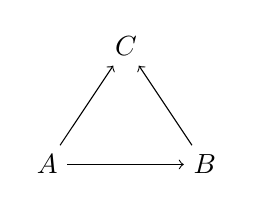
\begin{tikzpicture}
					% Nodes
					\node (A) at (0,0) {$A$};
					\node (B) at (2,0) {$B$};
					\node (C) at (1,1.5) {$C$};
					
					% Arrows
					\draw[->] (A) -- (B);
					\draw[->] (A) -- (C);
					\draw[->] (B) -- (C);
				\end{tikzpicture}
				
				% Commutative diagram
				\begin{tikzpicture}
					\matrix (m) [matrix of math nodes,
					row sep=3em, column sep=4em]{
						X & Y \\
						Z & W \\
					};
					\path[->]
					(m-1-1) edge (m-1-2)
					edge (m-2-1)
					(m-1-2) edge (m-2-2)
					(m-2-1) edge (m-2-2);
				\end{tikzpicture}
			\end{lstlisting}
		\end{column}
		
		\begin{column}{0.5\textwidth}
			\textbf{Basic diagram:}
			\begin{center}
				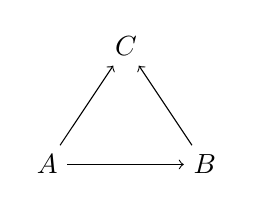
\begin{tikzpicture}
					% Nodes
					\node (A) at (0,0) {$A$};
					\node (B) at (2,0) {$B$};
					\node (C) at (1,1.5) {$C$};
					
					% Arrows
					\draw[->] (A) -- (B);
					\draw[->] (A) -- (C);
					\draw[->] (B) -- (C);
				\end{tikzpicture}
			\end{center}
			
			\textbf{Commutative diagram:}
			\begin{center}
				\begin{tikzpicture}
					\matrix (m) [matrix of math nodes,
					row sep=3em, column sep=4em]{
						X & Y \\
						Z & W \\
					};
					\path[->]
					(m-1-1) edge (m-1-2)
					edge (m-2-1)
					(m-1-2) edge (m-2-2)
					(m-2-1) edge (m-2-2);
				\end{tikzpicture}
			\end{center}
			
			\textbf{TikZ is powerful for:}
			\begin{itemize}
				\item Commutative diagrams
				\item Graphs and networks
				\item Geometric figures
				\item Custom illustrations
			\end{itemize}
		\end{column}
	\end{columns}
\end{frame}

\begin{frame}[fragile]{Custom Commands and Macros}
	\begin{columns}
		\begin{column}{0.5\textwidth}
			\begin{lstlisting}
				% In preamble
				% Simple command
				\newcommand{\R}{\mathbb{R}}
				\newcommand{\C}{\mathbb{C}}
				
				% Command with parameter
				\newcommand{\norm}[1]{\left\|#1\right\|}
				\newcommand{\set}[1]{\{#1\}}
				
				% Command with optional parameter
				\newcommand{\derivative}[2][x]{
					\frac{d #2}{d #1}
				}
				
				% In document
				Let $f: \R \to \R$ be a function.
				
				The norm $\norm{v}$ of vector $v$.
				
				The set $\set{1,2,3}$ contains 3 elements.
				
				$\derivative{f}$ and $\derivative[t]{f}$
			\end{lstlisting}
		\end{column}
		
		\begin{column}{0.5\textwidth}
			\textbf{Benefits of custom commands:}
			\begin{itemize}
				\item Consistent notation
				\item Shorter source code
				\item Easier to maintain
				\item Can modify once, affects all instances
			\end{itemize}
			
			\textbf{Command types:}
			\begin{itemize}
				\item \texttt{\textbackslash newcommand} - define new command
				\item \texttt{\textbackslash renewcommand} - redefine existing
				\item \texttt{\textbackslash providecommand} - only if not defined
			\end{itemize}
			
			\textbf{Parameters:}
			\begin{itemize}
				\item Mandatory: \texttt{[1]} - number of parameters
				\item Optional: \texttt{[1][default]} - with default
				\item Access with \texttt{\#1}, \texttt{\#2}, etc.
			\end{itemize}
		\end{column}
	\end{columns}
	
	\begin{tip}
		Define math commands in the preamble for consistent notation throughout your document
	\end{tip}
\end{frame}

\begin{frame}[fragile]{Common Errors and Debugging}
	\begin{columns}
		\begin{column}{0.5\textwidth}
			\textbf{Common error messages:}
			
			\begin{lstlisting}[language={}]
				! Undefined control sequence.
				l.10 \unkowncommand
				
			\end{lstlisting}
			\textcolor{red}{Typo or missing package}
			
			\begin{lstlisting}[language={}]
				! Missing $ inserted.
				l.15 The equation x^2
				
			\end{lstlisting}
			\textcolor{red}{Math command outside math mode}
			
			\begin{lstlisting}[language={}]
				! LaTeX Error: Environment unknown 
				undefined.
			\end{lstlisting}
			\textcolor{red}{Typo or missing package for environment}
			
			\begin{lstlisting}[language={}]
				! Missing \begin{document}.
				\end{lstlisting}
				\textcolor{red}{Text before \textbackslash begin\{document\}}
			\end{column}
			
			\begin{column}{0.5\textwidth}
				\textbf{Other common errors:}
				\begin{itemize}
					\item Missing or extra braces \{\}
					\item Unmatched environment \texttt{\textbackslash begin} / \texttt{\textbackslash end}
					\item Missing or mismatched \$ in math mode
					\item Undefined references or citations
					\item Package conflicts
				\end{itemize}
				
				\textbf{Debugging tips:}
				\begin{itemize}
					\item Look at line number in error message
					\item Comment out sections to isolate problems
					\item Add packages and commands incrementally
					\item Use \texttt{\textbackslash usepackage\{syntonly\}} to check syntax without output
					\item Use \texttt{\%} for comments to help debug
				\end{itemize}
			\end{column}
		\end{columns}
		
		\begin{warning}
			Always read the first error first - fixing it might solve later errors
		\end{warning}
	\end{frame}
	
	\begin{frame}[fragile]{Tips for Mathematical Writing}
		\begin{columns}
			\begin{column}{0.5\textwidth}
				\textbf{Spacing in math expressions:}
				
				\begin{lstlisting}
					% Too cramped
					$f(x)=x^2+2x+1$
					
					% Better with spacing
					$f(x) = x^2 + 2x + 1$
					
					% Manual spacing when needed
					\begin{align*}
						y &= x^2 \\
						&= (x+1)(x-1) + 1 \\
						&= x^2 - 1 + 1 \\
						&= x^2
					\end{align*}
					
					% Spacing commands
					$a \, b \: c \; d \! e$
					$p \quad q \qquad r$
				\end{lstlisting}
			\end{column}
			
			\begin{column}{0.5\textwidth}
				\textbf{Math spacing commands:}
				\begin{itemize}
					\item \texttt{\textbackslash,} - small space
					\item \texttt{\textbackslash:} - medium space
					\item \texttt{\textbackslash;} - large space
					\item \texttt{\textbackslash!} - negative space
					\item \texttt{\textbackslash quad} - 1em space
					\item \texttt{\textbackslash qquad} - 2em space
				\end{itemize}
				
				\textbf{Writing best practices:}
				\begin{itemize}
					\item Use punctuation in displayed equations
					\item Include math notation in the flow of text
					\item Be consistent with notation
					\item Define symbols when first introduced
					\item Use \texttt{\textbackslash text\{...\}} for text in math
					\item Avoid \texttt{\$\$...\$\$} (use \texttt{\textbackslash[...\textbackslash]} instead)
				\end{itemize}
			\end{column}
		\end{columns}
	\end{frame}
	
	\begin{frame}{Resources and Communities}
		\begin{columns}
			\begin{column}{0.5\textwidth}
				\textbf{Documentation:}
				\begin{itemize}
					\item \textbf{Books:}
					\begin{itemize}
						\item "The \LaTeX\ Companion" (Mittelbach et al.)
						\item "Mathematics into Type" (Swanson)
						\item "\LaTeX\ for Complete Novices" (Talbot)
					\end{itemize}
					
					\item \textbf{Online guides:}
					\begin{itemize}
						\item Overleaf Documentation
						\item CTAN package documentation
						\item LaTeX Wikibook
						\item TeX Stack Exchange tutorials
					\end{itemize}
				\end{itemize}
			\end{column}
			
			\begin{column}{0.5\textwidth}
				\textbf{Getting help:}
				\begin{itemize}
					\item TeX Stack Exchange
					\item r/LaTeX subreddit
					\item LaTeX Community forum
					\item Overleaf learn resources
				\end{itemize}
				
				\textbf{Useful tools:}
				\begin{itemize}
					\item Detexify - find symbols by drawing
					\item LaTeX Table Generator
					\item MathPix - convert images to LaTeX
					\item LaTeX templates (journals, theses)
				\end{itemize}
			\end{column}
		\end{columns}
		
		\begin{block}{Package documentation}
			Always check the documentation for packages you use:\\
			\texttt{texdoc packagename} (command line) or\\
			Visit \url{https://ctan.org/pkg/packagename}
		\end{block}
	\end{frame}
	
	\begin{frame}{Exercise 4: Final Document}
		\begin{practice}
			\textbf{Create a complete mathematical article that includes:}
			\begin{enumerate}
				\item Title, author, abstract
				\item Table of contents
				\item Mathematical content with properly typeset equations
				\item At least one theorem and its proof
				\item A figure or diagram
				\item A table
				\item Cross-references to all elements
				\item A bibliography with at least two references
			\end{enumerate}
		\end{practice}
		
		\textbf{Bonus goals:}
		\begin{itemize}
			\item Define a custom macro
			\item Include a TikZ diagram
			\item Format the document according to a journal style
		\end{itemize}
	\end{frame}
	
	\begin{frame}{Introduction to Beamer for Presentations}
		\begin{columns}
			\begin{column}{0.5\textwidth}
				\textbf{Beamer basics:}
				\begin{itemize}
					\item LaTeX document class for presentations
					\item Create professional slides with math
					\item Similar syntax to regular LaTeX
					\item Powerful theming and customization
				\end{itemize}
				
				\textbf{Key Beamer environments:}
				\begin{itemize}
					\item \texttt{frame} - individual slide
					\item \texttt{block}, \texttt{alertblock} - text boxes
					\item \texttt{columns} - multicolumn layout
					\item \texttt{itemize}, \texttt{enumerate} - lists
				\end{itemize}
			\end{column}
			
			\begin{column}{0.5\textwidth}
				\textbf{Themes and customization:}
				\begin{itemize}
					\item Presentation themes (Madrid, Berlin, etc.)
					\item Color themes (dolphin, crane, etc.)
					\item Font themes
					\item Inner/outer themes
				\end{itemize}
				
				\textbf{Special features:}
				\begin{itemize}
					\item Overlays and incremental builds
					\item Transitions and animations
					\item Notes for presenter
					\item Handout mode
				\end{itemize}
			\end{column}
		\end{columns}
		
		\begin{tip}
			This presentation was created with Beamer! You can look at the source code as a reference.
		\end{tip}
	\end{frame}
	
	\begin{frame}[fragile]{Basic Beamer Example}
		\begin{columns}
			\begin{column}{0.5\textwidth}
				\begin{lstlisting}
					\documentclass{beamer}
					\usetheme{Madrid}
					\usecolortheme{dolphin}
					
					\title{My Presentation}
					\author{Your Name}
					\date{\today}
					
					\begin{document}
						
						\\begin{frame}
						\titlepage
						\\end{frame}
						
						\\begin{frame}{Outline}
						\tableofcontents
						\\end{frame}
						
						\section{First Topic}
						
						\begin{frame}{Mathematics}
							The equation:
							\begin{equation}
								E = mc^2
							\end{equation}
							
							\begin{itemize}
								\item<1-> First point
								\item<2-> Second point
								\item<3-> Third point
							\end{itemize}
							\\end{frame}
							
							\\end{document}
						\end{lstlisting}
					\end{column}
					
					\begin{column}{0.5\textwidth}
						\textbf{Key points:}
						\begin{itemize}
							\item \texttt{\textbackslash documentclass\{beamer\}}
							\item Slides are created with \texttt{frame} environment
							\item Each frame needs a title with \texttt{\{title\}}
							\item \texttt{<1->} notation for incremental display
							\item All math commands work as usual
						\end{itemize}
						
						\textbf{Common elements:}
						\begin{itemize}
							\item Title page with \texttt{\textbackslash titlepage}
							\item Outline with \texttt{\textbackslash tableofcontents}
							\item Sections and subsections
							\item Math equations, tables, figures
						\end{itemize}
						
						
					\end{column}
				\end{columns}
			\end{frame}
			
			\begin{frame}{Workshop Summary}
				\textbf{What we've covered:}
				\begin{columns}
					\begin{column}{0.5\textwidth}
						\textbf{Hour 1: Getting Started}
						\begin{itemize}
							\item LaTeX basics and workflow
							\item Document structure
							\item Basic text formatting
							\item Lists and tables
						\end{itemize}
						
						\textbf{Hour 2: Mathematics}
						\begin{itemize}
							\item Inline and display math
							\item Math symbols and operators
							\item Matrices and alignment
							\item Multi-line equations
						\end{itemize}
					\end{column}
					
					\begin{column}{0.5\textwidth}
						\textbf{Hour 3: Document Structure}
						\begin{itemize}
							\item Theorems and proofs
							\item Figures and tables
							\item Cross-referencing
							\item Table of contents
						\end{itemize}
						
						\textbf{Hour 4: Advanced Topics}
						\begin{itemize}
							\item Bibliography
							\item Useful packages
							\item Debugging
							\item Beamer for presentations
						\end{itemize}
					\end{column}
				\end{columns}
				
				\begin{alertblock}{Next steps:}
					\begin{itemize}
						\item Practice regularly
						\item Explore advanced packages and features
						\item Use LaTeX for your research papers and presentations
						\item Join the LaTeX community
					\end{itemize}
				\end{alertblock}
			\end{frame}
			
			% Find this section at the end of your document
			\begin{frame}{Final Questions \& Discussion}
				\begin{center}
					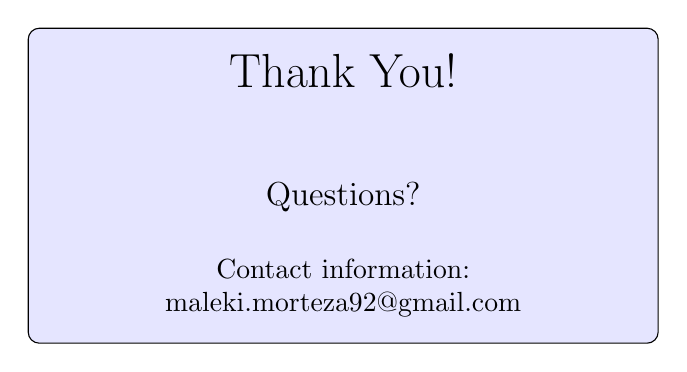
\begin{tikzpicture}
						\node[draw, rounded corners, fill=blue!10, minimum width=8cm, minimum height=4cm] {
							\begin{minipage}{7.5cm}
								\begin{center}
									\LARGE Thank You!
									
									\vspace{1cm}
									
									\large Questions?
									
									\vspace{0.5cm}
									
									\normalsize Contact information:\\ 
									maleki.morteza92@gmail.com
								\end{center}
							\end{minipage}
						};
					\end{tikzpicture}
				\end{center}
			\end{frame}


\end{document}